\documentclass[final]{fhnwreport}       %[mode] = draft or final
                                        %{class} = fhnwreport, article, 
                                        %          report, book, beamer, standalone
%%---Main Packages-----------------------------------------------------------------------
\usepackage[english, ngerman]{babel}	%Mul­tilin­gual sup­port for LaTeX
\usepackage[T1]{fontenc}				%Stan­dard pack­age for se­lect­ing font en­cod­ings
\usepackage[utf8]{inputenc}				%Ac­cept dif­fer­ent in­put en­cod­ings
\usepackage{lmodern}                    %The newer Font-Set
\usepackage{textcomp}					%LaTeX sup­port for the Text Com­pan­ion fonts
\usepackage{graphicx} 					%En­hanced sup­port for graph­ics
\usepackage{float}						%Im­proved in­ter­face for float­ing ob­jects
\usepackage{ifdraft}                    %Let you check if the doc is in draft mode

%%---Useful Packages---------------------------------------------------------------------
\usepackage[pdftex,dvipsnames]{xcolor}  %Driver-in­de­pen­dent color ex­ten­sions for LaTeX
\usepackage{csquotes}                   %Simpler quoting with \enquote{}
\usepackage{siunitx} 					%A com­pre­hen­sive (SI) units pack­age
\usepackage{listings}					%Type­set source code list­ings us­ing LaTeX
\usepackage[bottom]{footmisc}			%A range of foot­note op­tions
\usepackage{footnote}					%Im­prove on LaTeX's foot­note han­dling
\usepackage{verbatim}					%Reim­ple­men­ta­tion of and ex­ten­sions to LaTeX ver­ba­tim
\usepackage[textsize=footnotesize]{todonotes} %Mark­ing things to do in a LaTeX doc­u­ment

%%---Tikz Packages-----------------------------------------------------------------------
\usepackage{standalone}
\usepackage{tikz}
\usepackage{circuitikz}
\usetikzlibrary{arrows}
\usetikzlibrary{calc}
\usetikzlibrary{intersections}

%%---Math Packages-----------------------------------------------------------------------
\usepackage{amsmath}					%AMS math­e­mat­i­cal fa­cil­i­ties for LaTeX
%\usepackage{amssymb}					%Type­set­ting symbols (AMS style)
%\usepackage{array}						%Ex­tend­ing the ar­ray and tab­u­lar en­vi­ron­ments
%\usepackage{amsthm}					%Type­set­ting the­o­rems (AMS style)

%%---Table Packages----------------------------------------------------------------------
\usepackage{tabularx}					%Tab­u­lars with ad­justable-width columns
%\usepackage{longtable}
\usepackage{multirow}					%Create tab­u­lar cells span­ning mul­ti­ple rows
\usepackage{multicol}					%In­ter­mix sin­gle and mul­ti­ple columns

%%---PDF / Figure Packages---------------------------------------------------------------
\usepackage{pdfpages}					%In­clude PDF doc­u­ments in LaTeX
\usepackage{pdflscape}					%Make land­scape pages dis­play as land­scape
\usepackage{subfig}					    %Fig­ures di­vided into sub­fig­ures

%%---Other Packages----------------------------------------------------------------------
%\usepackage{xargs}                     %De­fine com­mands with many op­tional ar­gu­ments

%%---Bibliography------------------------------------------------------------------------
\usepackage[style=ieee,urldate=comp,backend=biber]{biblatex}
\addbibresource{literature/bibliography.bib}

%%---Main Settings-----------------------------------------------------------------------
\graphicspath{{./graphics/}}			%Defines the graphicspath
%\geometry{twoside=false}				    %twoside=false disables the "bookstyle"
\setlength{\marginparwidth}{2cm}
\overfullrule=5em						%Creates a black rule if text goes over the margins => debugging


%%---User Definitions--------------------------------------------------------------------
%%Tabel-Definitions: (requires \usepackage{tabularx})
\newcolumntype{L}[1]{>{\raggedright\arraybackslash}p{#1}}    %column-width and alignment
\newcolumntype{C}[1]{>{\centering\arraybackslash}p{#1}}
\newcolumntype{R}[1]{>{\raggedleft\arraybackslash}p{#1}}

%%---Optional Package Settings-----------------------------------------------------------
%Listings-Settings: (requires \usepackage{listings}) => Example with Matlab Code
\lstset{language=Matlab,%
    basicstyle=\footnotesize\ttfamily,
    breaklines=false,%
    morekeywords={switch, case, otherwise},
    keywordstyle=\color{Blue},%
    tabsize=2,
    %morekeywords=[2]{1}, keywordstyle=[2]{\color{black}},
    identifierstyle=\color{Black},%
    stringstyle=\color{Purple},
    commentstyle=\color{Green},%
    showstringspaces=false,%without this there will be a symbol in the places where there is a space
    numbers=left,%
    numberstyle={\tiny \color{black}},% size of the numbers
    numbersep=9pt, % this defines how far the numbers are from the text
    %emph=[1]{word1, word2,...},emphstyle=[1]\color{red}
}										                %loads all packages, definitions and settings												
\title{Der Einstieg in \LaTeX}          %Project Title
\author{Vorlage und Beispiele}          %Document Type => Technical Report, ...
\date{Windisch, 13.08.2018}             %Place and Date

\begin{document}

%%---TITLEPAGE---------------------------------------------------------------------------
\selectlanguage{ngerman}                %ngerman or english
\maketitle

\vspace*{-1cm}						    %compensates the space after the date line.
\vfill
\begin{figure}[H]
\centering

\includegraphics[width=\linewidth]{titelbild.pdf}
\end{figure}
\vfill

{
\renewcommand\arraystretch{2}
\begin{center}
\begin{tabular}{>{\bf}p{4cm} l}
Hochschule                 &    Hochschule für Technik - FHNW\\
Studiengang                &    Elektro- und Informationstechnik\\
Autor   		           & 	Patrick Studer und Hanspeter Schmid\\
Betreuer                   &    Anita Gertiser\\
Auftraggeber               &    Sebastian Gaulocher\\
Version                    &    1.2 %Normally not used!
\end{tabular}
\end{center}
}

\clearpage
			
%%---ABSTRACT----------------------------------------------------------------------------
\selectlanguage{ngerman}				%ngerman or english
\thispagestyle{empty}
\begin{abstract}
Das Abstract ist eine Art Zusammenfassung des ganzen Dokuments. Es gibt einen Einblick in die Aufgabenstellung, wie diese umgesetzt wurde und welches Ergebnis erreicht wurde. Aus diesem Grund wird das Abstract immer ganz am Schluss der Arbeit verfasst. Es besteht aus einem zusammengehörenden Absatz und umfasst ungefähr 10 bis 20 Zeilen.
Formeln, Referenzen oder andere Unterbrechungen haben im Text nichts zu suchen.
Direkt unter dem Abstract folgt eine Liste von drei bis vier Stichworten/Keywords. Diese werden in alphabetischer Reihenfolge aufgelistet und beschreiben das Themengebiet der Arbeit.

\vspace{2ex}
\textbf{Keywords: Anleitung, LaTeX, Thesis, Vorlage}
\end{abstract}	


\vfill

\begin{center}
\color{green!50!black!100}\bf
Bitte schicken Sie jeglichen Feedback auch an \texttt{hanspeter.schmid@fhnw.ch}\\
Er wird dieses Template langfristig unterhalten.
\end{center}

\vfill
\null

%%---TABLE OF CONTENTS-------------------------------------------------------------------
\pagenumbering{Roman}		
\selectlanguage{ngerman}				%ngerman or english
\tableofcontents
\clearpage

%%---TEXT--------------------------------------------------------------------------------
\pagenumbering{arabic}
\section{Grundlagen}
Diese Vorlage soll den Studenten im Studiengang Elektro- und Informationstechnik den Einstieg in \LaTeX\ vereinfachen und anhand von Beispielen \textbf{(siehe direkt im tex-File)} einige Tipps und Tricks auf den Weg geben. Zudem wird auch auf Vorgaben eingegangen, welche für eine technische Dokumentation wichtig sind und sicherstellen, dass alle Dokumentationen des Studiengangs gleich designed werden. Für \LaTeX "~Neulinge wird das Dokument \emph{LaTeX2e-Kurzbeschreibung} (siehe \cite{l2kurz}) empfohlen.  Die elektronische Datei ist im Ordner \mbox{\emph{/bibliography/}} zu finden. Daraus stammt auch das folgende Zitat:
\begin{quote}
Typographisches Design ist ein Handwerk, das erlernt werden muss. Ungeübte Autoren machen dabei oft gravierende Fehler. Fälschlicherweise glauben viele Laien, dass Textdesign vor allem eine Frage der Ästhetik ist -- wenn das Schriftstück vom künstlerischen Standpunkt aus \enquote{schön} aussieht, dann ist es schon gut \enquote{designed}. Da Schriftstücke jedoch gelesen und nicht in einem Museum aufgehängt werden, sind die leichtere Lesbarkeit und bessere Verständlichkeit wichtiger als das schöne Aussehen. \cite{l2kurz}
\end{quote}

\subsection{Teamfähige Installation}

Bei der Arbeit mit \LaTeX{} empfiehlt es sich sehr, dass alle im Team dieselbe Version installiert haben.  Am einfachsten ist das mit einer Installation von \url{https://tug.org/texlive/}.  Dies ist eine nahezu vollständige Installation von allem was es braucht, so aufbereitet, dass die Dateiversionen zusammenpassen, und lauffähig auf Linux, MacOS und Windows.

\subsection{Grundgerüst}
Um ein \LaTeX-Dokument zu erstellen braucht es eigentlich nicht viel, nur eine Textdatei mit der Dateiendung \texttt{.tex}, welche mit dem Befehl \verb|\documentclass[]{}| beginnt und die Umgebung \verb|\begin{document}| \dots \verb|\end{document}| enthält.
Darin kann nun die ganze Dokumentation erstellt und kompiliert werden, jedoch wird das schnell unübersichtlich und eignet sich sehr schlecht für das gemeinsame Arbeiten am Dokument.

Durch das "`Outsourcen"' von zusammengehörenden Blöcken (z.\,B. ganze Kapitel) in externe Dateien kann eine \textbf{übersichtliche und teamfähige Struktur} geschaffen werden. Damit sie bei der Kompilation des Dokuments beachtet werden, müssen sie in der Masterdatei eingebunden werden.
Einerseits wird der Befehl \verb|\input{}| dazu verwendet, Texte \textbf{1:1} aus einer Datei einzubinden. Dies kann beispielsweise dazu dienen, die Dokumenteinstellungen und Packages aus einer externen Datei (hier \mbox{\texttt{header.tex}}) zu laden.\footnote{Beim Kompiliervorgang wird das aktuelle \texttt{.aux}"~File weitergeführt.}
Andererseits können ganze Kapitel mit \verb|\include{}| eingebunden werden. Dieser Befehl fügt ein zusätzliches \verb|\clearpage| \textbf{vor} und \textbf{nach} dem geladenen Text hinzu. Dadurch wird sichergestellt, dass ein Seitenumbruch am Anfang und Schluss gesetzt und die Gleitobjekt"=Warteschlange geleert wird.\footnote{Für das eingefügte Kapitel wird ein separates \texttt{.aux}"~File erzeugt.} Zu beachten ist, dass der \verb|\include{}|"~Befehl nur in der Masterdatei benutzt wird, da er nicht verschachtelt werden kann. 

In Abbildung~\ref{fig:Struktur} ist die Struktur des aktuellen \LaTeX-Projekts aufgezeigt.\\
\textbf{Diese Struktur ist als Minimalstruktur zu verstehen und ist für Berichte des Studiengangs EIT vorgeschrieben!}

\clearpage 

Die Ordner sind für folgende Dateien vorgesehen:
\begin{tabbing}
\quad \= \verb|appendix/| \qquad \= im Anhang eingebundene Dokumente oder Bilder\\
      \> \verb|graphics/|        \> Grafiken (vorzugsweise als Vektorgrafik -- pdf)\\
      \> \verb|literature/|      \> zitierte Dokumente, Paper, Webseiten und die Bibliographie-Datenbank\\
      \> \verb|sections/|        \> mit \verb|\include{section.tex}| eingefügte Kapitel\\
      \> \verb|tikz/|            \> tikz-Grafiken (Standalone-Modus) zum Einbinden mit \verb|\section{Tikz-Grafiken}
Tikz ist ebenfalls sehr mächtig und auf den ersten Blick auch sehr kompliziert. Schon alleine die Dokumentation des Grundpackages erstreckt sich über 1000 Seiten. Tikz lohnt sich vor allem, wenn die erstellte Grafik (oder nur Teile davon) wiederverwendet werden können.
Es folgen drei Beispiele für Tikz-Grafiken.

Man beachte, dass diese in einem eigenen \enquote{\LaTeX-Projekt} erstellt wurden. Dieses hat die \verb|\documentclass{standalone}| und kann deswegen eigenständig kompiliert werden. Dabei werden automatisch Unterstüzungslinien/Grid eingeblendet (wurde programmiert), welche die Gestaltung der Grafik extrem erleichtern. Schaut euch doch die Tikz-Dateien an und kompiliert sie separat, es lohnt sich!

Mittels Befehl \verb|\includestandalone{}| werden dann diese in jedes andere Projekte eingebunden, und zwar nicht als PDF sondern direkt erstellt beim Kompilieren.

Somit können wir nun einfache elektrische Schaltungen wie in Figur~\ref{subfig:einfach} oder auch komplizierte Blockschaltbilder wie in Figur~\ref{subfig:kompliziert} programmieren.

\begin{figure}[b]
\centering
\subfloat[Einfach]{\includestandalone{tikz/beispiel1}\label{subfig:einfach}}

\subfloat[Kompliziertes Blockschaltbild]{\includestandalone{tikz/beispiel2}\label{subfig:kompliziert}}

\caption{Zwei tikz-Beispiele: \protect\subref{subfig:einfach} einfach, \protect\subref{subfig:kompliziert} kompliziert.}
\label{fig:tikz}
\end{figure}

Im Dokumenteordner \mbox{\emph{/tikz/}} findet ihr noch zwei weitere Beispiele. Eines zeigt ein \textbf{animiertes Tikz} und das andere interagiert mit \textbf{gnuplot}, um Plots zur Laufzeit zu erstellen. Um gnuplot nutzen zu können sind ein paar zusätzliche Installationen notwendig. Weiter muss der Kompilierbefehl für \texttt{pdflatex} mit \texttt{--shell-escape} erweitert werden. Das Internet bietet gute Unterstützung bei der Integration von gnuplot.
Viele weitere coole Beispiele findet ihr auf \mbox{http://www.texample.net/tikz/examples/}.

|\\
      \> \verb|versions/|        \> Ablage für verschiedene Dokumentversionen (z.\,B. bei Abgabe)
\end{tabbing} 

\begin{figure}
\centering
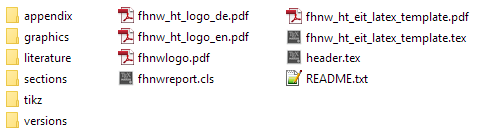
\includegraphics[width=0.8\linewidth]{ordner_struktur.png}
\caption{Minimalstruktur des \LaTeX -Projekts.}\label{fig:Struktur}
\end{figure}

\subsection{Packages}
Packages können dem Benutzer helfen, gewisse Dinge einfacher zu Programmieren, indem vorgefertigte Funktionen geladen werden. Dies ist zwar nützlich, sollte jedoch mit Vorsicht genossen werden.
\textbf{Unterschiedliche Packages können einander gegenseitig beeinflussen und dadurch unerklärliche Fehler verursachen. Aus diesem Grund empfiehlt sich, nur wirklich verwendete Packages dem Header hinzufügen!}
Auch bei Beispielen aus dem Internet ist immer etwas Vorsicht geboten. Viele Examples binden unnötige Packages ein. Am besten also alle ungebrauchten Packages im Header auskommentieren und erst wieder einkommentieren, wenn der Kompiler meckert, dass er ein Befehl nicht kennt.

\subsection{Gliederung}
Die \texttt{fhnwreport}-Klasse basiert auf der \LaTeX -Klasse \texttt{article}. Für die Gliederung können drei nummerierte und eine nicht nummerierte Ebenen verwendet werden. Da unsere Berichte nicht mehrere Hundert Seiten beinhalten, sind Kapitelseiten (\verb|\chapter{}|) nicht vorgesehen. Somit wird mittels \verb|\section{}| die oberste Gliederungsebene angesprochen. Mittels \verb|\subsection{}| resp. \verb|\subsubsection{}| werden die nächsten zwei Ebenen definiert. 

\paragraph{Das ist ein Paragraph}
Ein Paragraph kann mit dem Befehl \verb|\paragraph{}| erstellt werden und wird nicht im Inhaltsverzeichnis aufgelistet. Es setzt nur einen fetten Titel und beginnt danach auf einer neuen Zeile.

\subsubsection{Tiefe des Inhaltsverzeichnis beschränken}
Das Inhaltsverzeichnis ist durch die Klasse auf eine Tiefe von drei Ebenen eingestellt. Nun kann es vorkommen, dass man in einem Kapitel die unterste Ebene ausblenden möchte, jedoch nicht auf die nummerierten Überschriften verzichten möchte.
Dies kann einfach gemacht werden, indem man mit dem Befehl \verb|\addtocontents{toc}{\protect\setcounter{tocdepth}{2}}| die Tiefe auf Ebene~2 setzt. Die darauf folgenden Überschriften der 3. Ebene sind dann nicht mehr im Inhaltsverzeichnis aufgelistet. 

\addtocontents{toc}{\protect\setcounter{tocdepth}{2}}

\subsubsection{Dieser Titel ist nicht im Inhaltsverzeichnis}
Am Schluss muss jedoch die Tiefe wieder zurück auf die Standardeinstellung gesetzt werden (\verb|\addtocontents{toc}{\protect\setcounter{tocdepth}{3}}|), damit im nächsten Kapitel wieder alle Gliederungsebenen angezeigt werden.

\addtocontents{toc}{\protect\setcounter{tocdepth}{3}}

\subsection{Kommentare}\label{sec:todos}
Möchte man Kommentare setzen kann dies einfach mit dem Package \texttt{todonotes} realisiert werden. Die Kommentare können mit dem Befehl \verb|\todo{}| am Seitenrand oder für längere Kommentare mit \verb|\todo[inline]{}| direkt im Text angeordnet werden. \todo{Todo am Seitenrand}
\todo[inline]{Todo im Text}

Das Wichtigste jedoch ist, vor Abgabe alle Todo's abgearbeitet zu haben. Dabei hilft ein weiteres schönes Feature -- die \verb|\listoftodos|. Sie bietet eine Übersicht über alle definierten Todo’s. Ähnlich wie beim Inhaltsverzeichnis braucht diese Liste zwei Kompilierdurchgänge. Aktuell wird sie nur erstellt, solange das Dokument im \texttt{mode=draft} ist (siehe am Schluss des Hauptdokuments).

\subsection{Verweise}
Verweise helfen dem Leser, Zusammenhänge zwischen verschiedenen Themen besser zu erkennen. Die Verweise auf andere Kapitel wie z.\,B. (siehe Kapitel~\ref{sec:todos}) können nach eigenem Ermessen platziert werden. \textbf{Verweise auf Abbildungen und Tabellen sind jedoch Pflicht!} Das Dokument darf keine Bilder oder Tabellen enthalten, ohne dass im dazugehörigen Abschnitt darauf referenziert wird.

\subsubsection{Label setzen}
Um auf etwas verweisen zu können, muss zuerst ein Label gesetzt werden. Dies wird mit dem Befehl \verb|\label{}| gemacht. Den Befehl setzt man direkt hinter Überschriften oder hinter die Beschreibung (\verb|\caption{}|) von Abbildungen und Tabellen.  Die Funktion von \verb|\label{}| ist ganz einfach: der Befehl speichert die letzte automatisch erzeugte Nummer ab, was immer das auch war. Deshalb ist im obigen Text das Wort \textbf{nach} ganz besonders wichtig.

Grundsätzlich können die Labels beliebig benannt werden. Jedoch ist es für die Teamarbeit oder auch für eure Nachfolger extrem hilfreich, wenn ein einheitliches Namenssystem eingehalten wird. \textbf{Deshalb gilt für Dokumentationen des Studiengangs EIT folgende Richtlinie für die Vergabe von Labelnamen:}
\begin{tabbing}
\quad \= \verb|\label{sec:name}|  \qquad \= für Kapitel (sections)\\
      \> \verb|\label{fig:name}|  \> für Bilder (figures)\\
      \> \verb|\label{tab:name}|  \> für Tabellen (tables)\\
      \> \verb|\label{equ:name}|  \> für Formeln (equations)\\
      \> \verb|\label{app:name}|  \> für Objekte im Anhang (appendix)
\end{tabbing}

\subsubsection{Auf Labels referenzieren}
Wurde erstmal ein Label gesetzt, kann von einer beliebigen Stelle im Dokument darauf referenziert werden. Dazu kann man zwei Befehle nutzen: \verb|\ref{}| und \verb|\pageref{}|. Zu beachten ist, dass diese Befehle nur eine Zahl (Index oder Seite) des Objektes zurückgeben. Damit die Formelreferenz automatisch in runde Klammern gesetzt wird, bietet sich der Befehl \verb|\eqref{}| an. Referenzen werden erst nach \textbf{zwei Kompilierdurchgängen} richtig angezeigt.

\subsection{Abstände, Bindestriche und Silbentrennung}
Die wichtigsten Befehle für horizontale Abstände sind:
\begin{tabbing}
\quad \= \verb|\phantom{}| \qquad \= \kill
      \> \verb|~|          \> Leerschlag~mit~unterdrücktem~Zeilenumbruch \\
      \> \verb|\,|         \> Kleiner\,Abstand \\
      \> \verb|\;|         \> Mittelgrosser\;Abstand \\
      \> \verb|\!|         \> Den\!Abstand\!verkürzen (kann auch mehrmals angewendet werden: zum\!\!\!Beispiel) \\
      \> \verb|\quad|      \> Abstand\quad so\quad breit\quad wie\quad ein\quad Buchstabe\quad hoch\quad ist \\
      \> \verb|\qquad|     \> Doppelter\qquad \verb|\quad| \\
      \> \verb|\enspace|   \> So breit wie eine Ziffer (123\enspace 56\enspace 8) \\
      \> \verb|\phantom{}| \> So breit wie der übergebene Text (Das ist ein \phantom{Phantom}-Beispiel)\\
      \> \verb|\hspace{}|  \> So breit wie man will (Das sind 2\,cm\hspace{2cm}Abstand)\\
      \> \verb|\hfill|     \> Abstand, bis die Zeile voll ist \\
      \> \verb|\dotfill|   \> Punkte, bis die Zeile voll ist \\
      \> \verb|\hrulefill| \> Linie, bis die Zeile voll ist \\
\end{tabbing}

Die wichtigsten Befehle für vertikale Abstände sind:
\begin{tabbing}
\quad \= \verb|\phantom{}| \qquad \= \kill
      \> \verb|\smallskip| \> Kleiner Abstand\\
      \> \verb|\medskip|   \> Mittlerer Abstand\\
      \> \verb|\bigskip|   \> Grosser Abstand\\
      \> \verb|\parskip|   \> Definierter Absatzabstand\\
      \> \verb|\vphantom|  \> So hoch wie der übergebene Text (hilfreich in Formeln)\\
      \> \verb|\vspace{}|  \> So hoch wie man will\\
      \> \verb|\vfill|     \> Abstand, bis die Seite voll ist\\
\end{tabbing}

Für Minuszeichen, Bindestriche und Gedankenstriche wird in Latex das selbe Symbol verwendet:
\begin{tabbing}
\quad \= \verb|\phantom{}| \qquad \= \kill
      \> \verb|$-$|        \> Mathematisches Minus: $1-2=-1$ \\
      \> \verb|-|          \> Bindestrich: O-Beine, AD-Wandler \\
      \> \verb|"~|         \> Bindestrich der nicht unterbrochen werden darf \\
      \> \verb|--|         \> Gedankenstriche: Ja -- oder doch nein? \\
      \>                   \> Bis/Nach: 11--18~Uhr, Zürich--Paris \\
      \>                   \> Versus: Basel -- Zürich \\
      \> \verb|---|        \> Langer Gedankenstrich ohne Abstand (nur im Englischen): yes---or no?\\
\end{tabbing}

Möchte man die automatische Silbentrennung von \LaTeX{} beeinflussen helfen folgende Befehle:
\begin{tabbing}
\quad \= \verb|\phantom{}| \qquad \= \kill
      \> \verb|\-|         \> Dieses Wort darf nur an dieser Stelle \\
      \>                   \> oder nach einem Bindestrich getrennt werden\\
      \> \verb|"-|         \> Diesem Wort eine zusätzliche Trennstelle hinzufügen \\
      \> \verb|\mbox{}|    \> Dieser Satz wird weder umgebrochen, noch werden die Wörter getrennt\\
      \> \verb|\hyphenation{}| \> Die aufgelisteten Wörter dürfen im gesamten Dokument \\
      \>                   \> nur an den mit \verb|-| markierten Stellen getrennt werden\\
\end{tabbing}

\clearpage

\subsection{Zahlen und Einheiten}
Um die Abstände zwischen Zahlen und deren Einheitsangabe richtig darzustellen bietet sich das Package \verb|siunitx| an. Es hilft bei Angaben von Einheiten, Zahlenbereichen oder Zehnerpotenzen.

Die Zahlen \texttt{1234} und \texttt{1.234e3} können mit \verb|\num{}| angezeigt werden. Für Winkel wie $45^\circ$ oder $60^\circ20'10''$ verwenden wir \verb|\ang{}|.
Für alleinstehende Einheiten wie \texttt{km/h} oder \texttt{m/s\string^2} gibt es den \verb|\si{}|-Befehl, und schlussendlich bildet die Kombination aus \verb|\num{}| und \verb|\si{}| den Befehl \verb|\SI{}{}|.
{
\sisetup{
list-final-separator = { und },
list-pair-separator = { und },
range-phrase = { bis },
}

Beispiele: \num{1234} ist gleichviel wie \num{1.234e3}. \SI{2}{\pi} sind \ang{360;0;0}. \numlist{1;2;3;4;5} sind Zahlen von \numrange{1}{5}. \si{kg.m/s^2} sind \si{\kilo\gram\per\square\second}. \SI{112}{km/h} oder \SI{112}{\kilo\meter\per\hour}.

\subsection{Sprache umstellen}
Man kann an einer beliebigen Stelle im Dokument die Sprache wechseln. Dies bewirkt, dass automatisch generierte Texte in der jeweiligen Sprache eingefügt werden. Der Befehl dazu lautet \verb|\selectlanguage{ngerman}| für Deutsch und \verb|\selectlanguage{english}| für Englisch.


\section{Gleitobjekte (floats)}
Im Normalfall werden Objekte nicht genau dort im Text platziert, wo sie inhaltlich auch hingehören. \LaTeX{} versucht viele typographische Regeln zu erfüllen, um ein \enquote{korrektes} Schriftbild zu erreichen. Diese Regeln schaffen etwas Freiraum und erhöhen die Lesefreundlichkeit. Deshalb werden Tabellen und Abbildungen automatisch an die nächstmögliche geeignete Stelle \enquote{gleiten} und nachfolgende Objekte vor sich her schieben (quasi eine Warteschlange), bis das Dokument zu ende ist oder der Befehl \verb|\clearpage| eingegeben wird.

Um so eine Gleitumgebung zu schaffen stellt \LaTeX{} die beiden Umgebungen \texttt{figure} und \texttt{table} zur Verfügung. Bei Blocksatz ist es also so, dass Bilder und Tabellen am oberen oder unteren Blattrand, oder auf einer eigenständigen Seite (ohne Text) platziert werden. Dies, weil der Float-Specifier ohne Angabe auf \texttt{[tbp]} gesetzt ist (top, bottom, page). \textbf{Dies sollte immer die erste Wahl sein.}

Hat man jedoch sehr viele Bilder oder ist mit den automatisch gesetzten Bildpositionen nicht einverstanden, so ist eine Nachbearbeitung ganz am Schluss sinnvoll.
Durch Setzen von \texttt{[t]} oder \texttt{[b]} kann nach Belieben eingegriffen werden.
Sollte das immer noch nicht reichen können durch ein zusätzliches \texttt{!} (bang) die \LaTeX-Regeln für den Mindestanteil an normalem Text pro Seite umgangen werden.

\subsection{Abbildungen (figure)}
Eine Abbildung beginnt mit \verb|\begin{figure}| und endet mit \verb|\end{figure}|.
Dazwischen stehen Anweisungen für das Hinzufügen der Grafik, der Bildunterschrift und des Labels für die Referenzierung. Oft wird der Parameter \texttt{size=faktor} verwendet. Dieser hat jedoch den Nachteil, dass er abhängig von der Originalgrösse der Grafik ist. Besser ist die Verwendung des Parameters \texttt{width}. Dazu folgendes Beispiel, welches der Abbildung~\ref{fig:Figure} entspricht:

\begin{verbatim}
\begin{figure}[b]
  \centering
  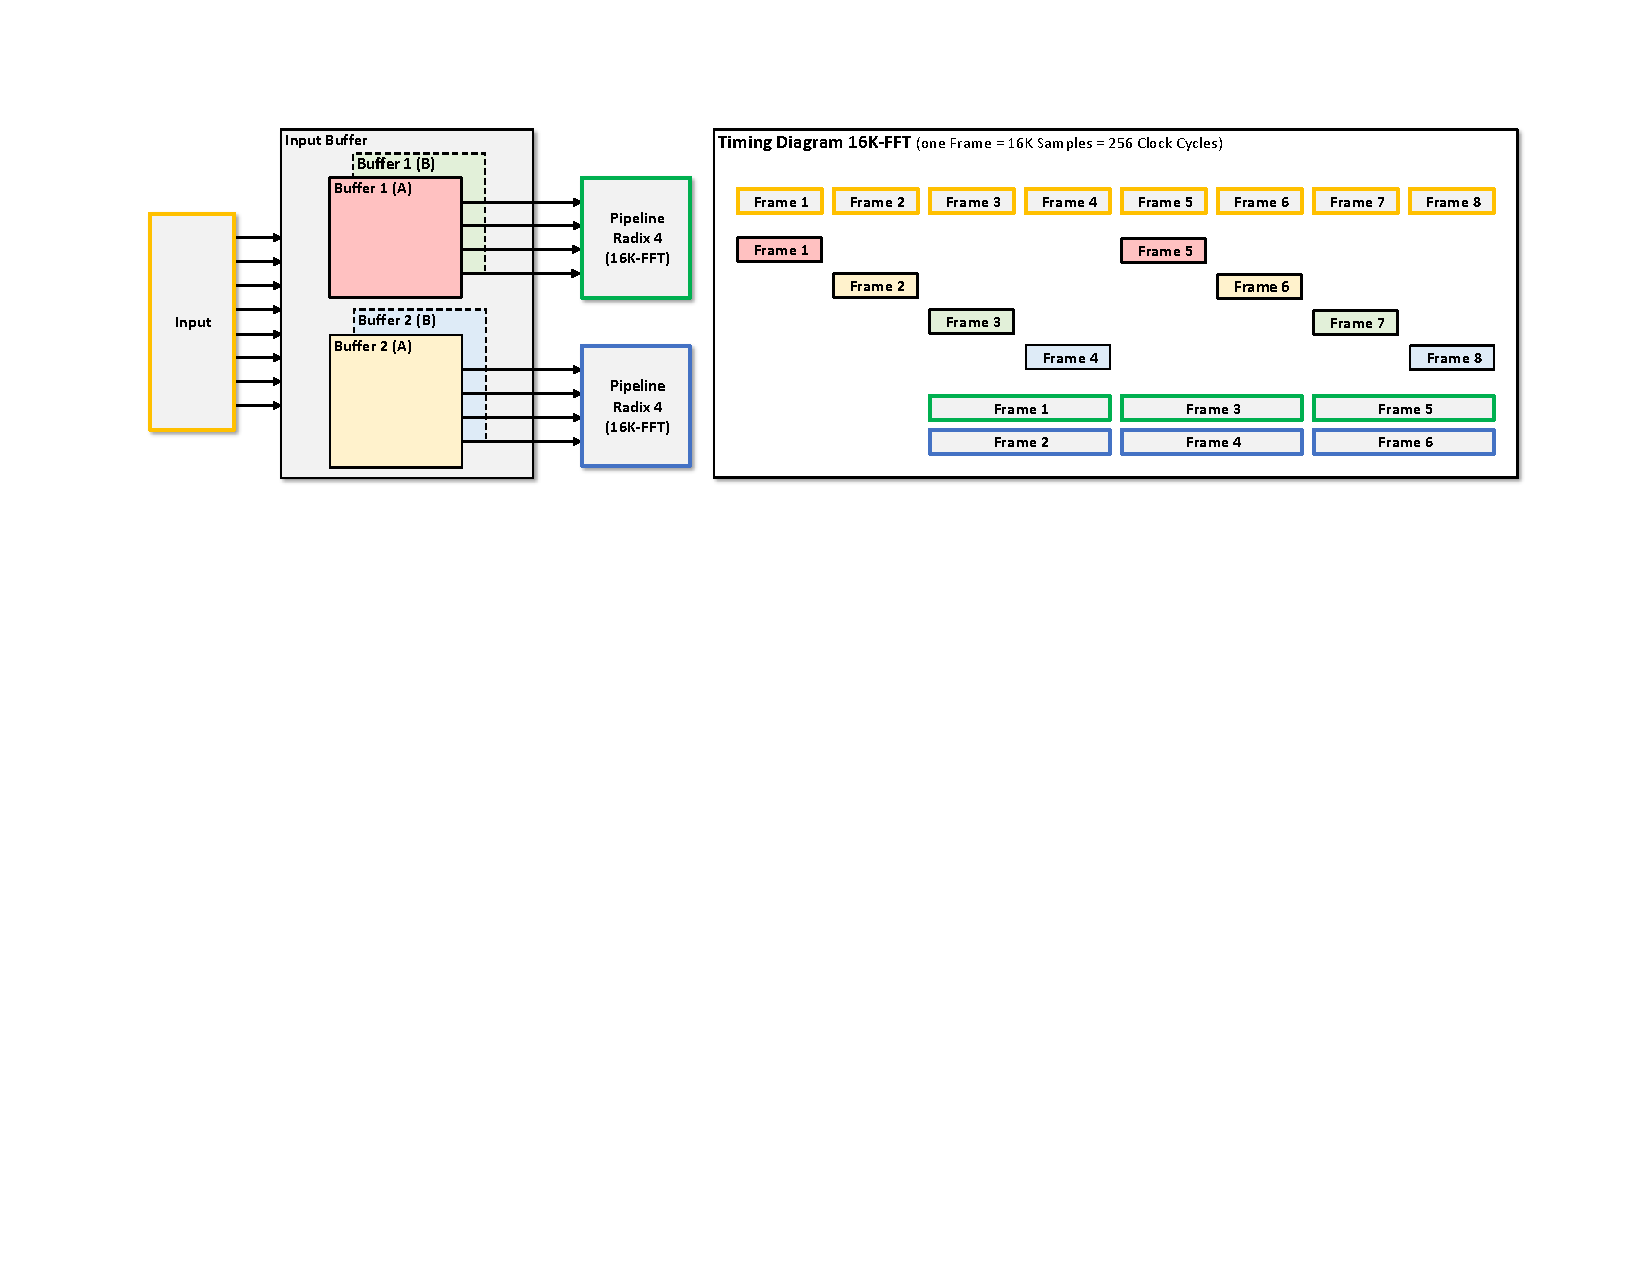
\includegraphics[width=0.9\linewidth]{beispiel.pdf}
  \caption{Dies ist ein Beispiel für eine Abbildung.}
  \label{fig:Figure}
\end{figure}
\end{verbatim}

\begin{figure}[b]
\centering
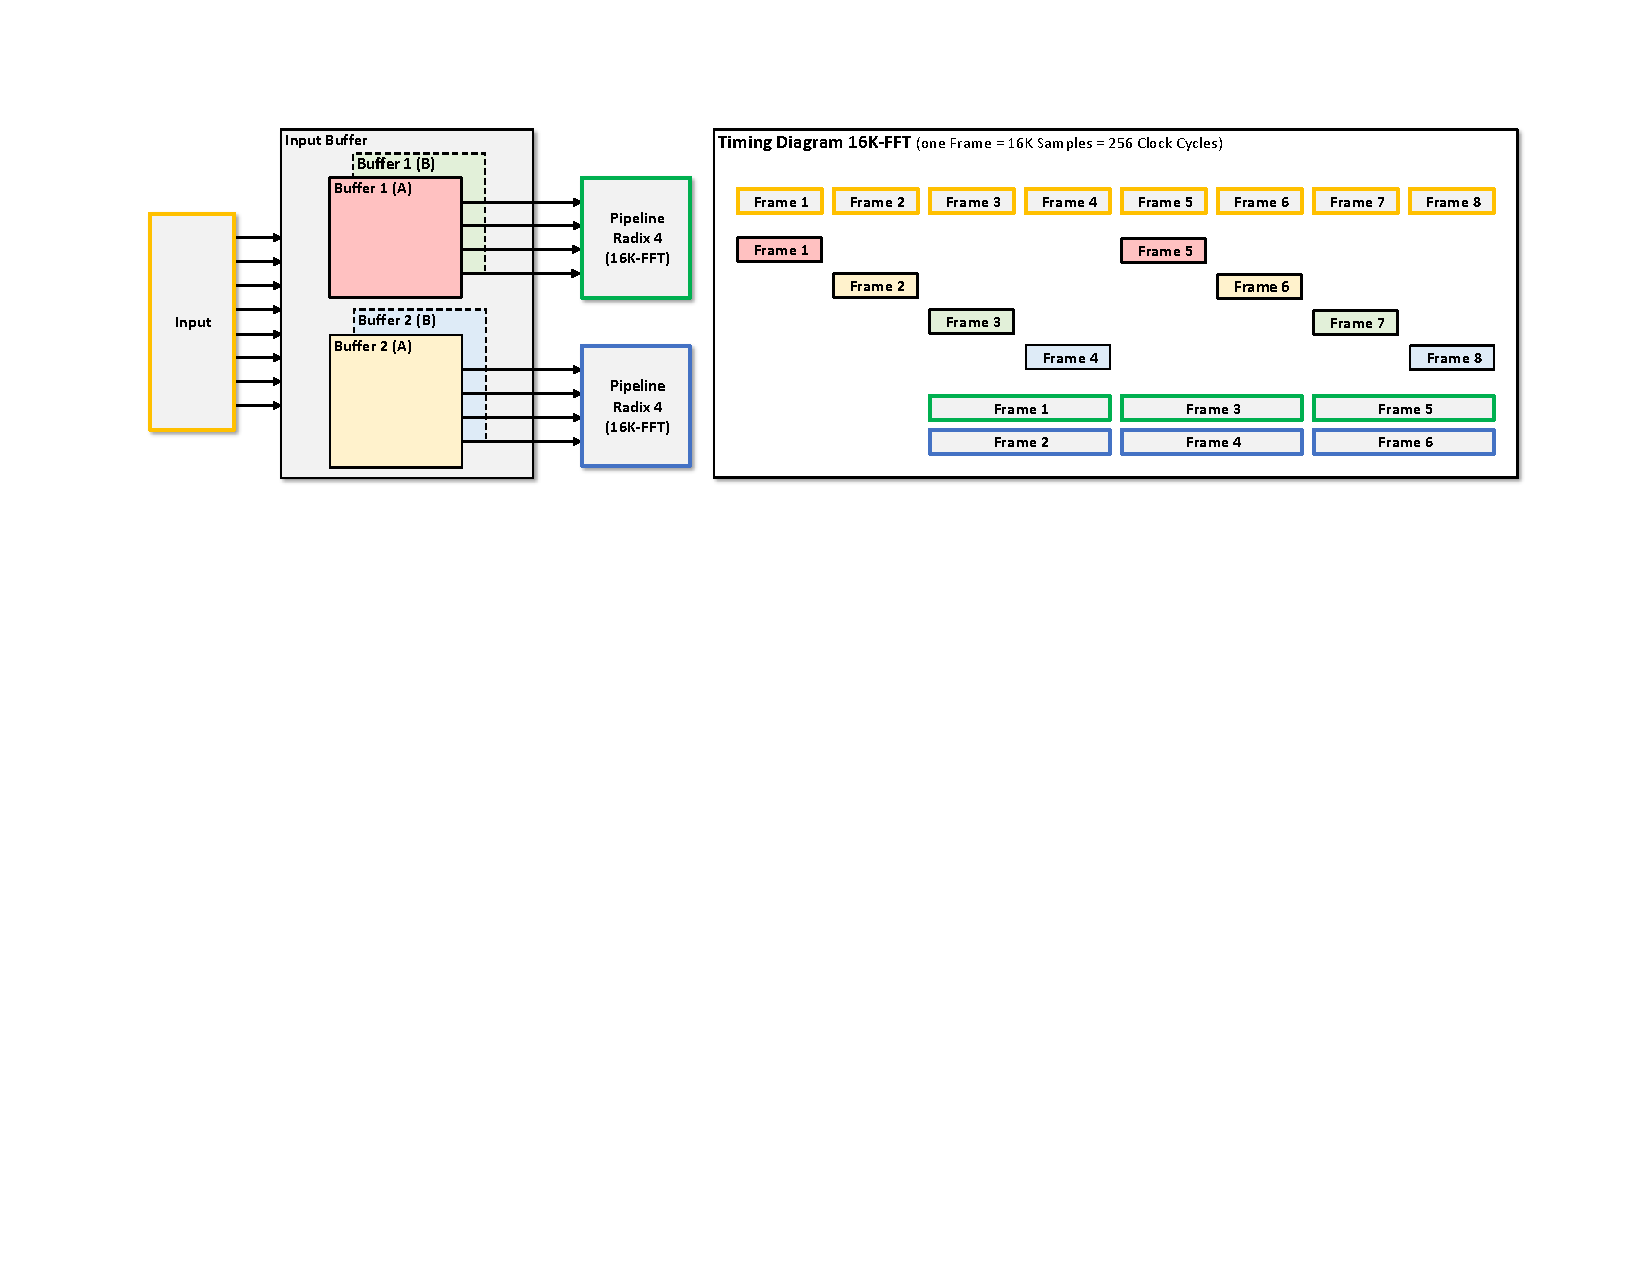
\includegraphics[width=0.9\linewidth]{beispiel.pdf}
\caption{Dies ist ein Beispiel für eine Abbildung.}
\label{fig:Figure}
\end{figure}

\subsubsection{Subfigures}
Hat man mehrere kleine Bilder (die irgendwie zusammengehören), kann man diese platzsparend in einer Subfigure anordnen. In Abbildung~\ref{fig:Subfigure} auf Seite~\pageref{fig:Subfigure} sieht man ein kleines Beispiel von Subfigures. Für diese wird das Package \verb|subfig| verwendet.

\begin{figure}[t]
\centering
\subfloat[Bild 1]{\rule{4cm}{3cm}}\qquad
\subfloat[Bild 2]{\rule{4cm}{3cm}}\qquad
\subfloat[Bild 3]{\rule{4cm}{3cm}}
\caption{Ein einfaches Beispiel für eine Abbildung mit mehreren Bildern.}
\label{fig:Subfigure}
\end{figure}

\subsection{Tabellen (table)}
Eine Tabellen beginnt mit \verb|\begin{table}| und endet mit \verb|\end{table}|.
Dazwischen stehen Anweisungen für das Erstellen der eigentlichen Tabellenanordnung, die Tabellenbeschreibung und ein Label für die Referenzierung. Dazu ein Beispiel, welches der Tabelle~\ref{tab:Table1} entspricht:

\begin{table}[b]
\centering
\begin{tabular}{C{1cm} C{2.5cm} C{2cm}|C{2cm} C{2.5cm} C{1cm}} 
\multicolumn{3}{c|}{\textbf{Normally Ordered Input}} & \multicolumn{3}{c}{\textbf{Digit-Reversed Output}} \\
{Index} & {Base 2} & {Base 4} & {Base 4} & {Base 2} & {Index} \\ \hline\hline 
60    &   11 11 00    & 330    & 033    & 00 11 11    &    15\\
61    &   11 11 01    & 331    & 133    & 01 11 11    &    31\\
62    &   11 11 10    & 332    & 233    & 10 11 11    &    47\\
63    &   11 11 11    & 333    & 333    & 11 11 11    &    63\\
\end{tabular}
\caption{Das erste Beispiel für eine Tabelle.}
\label{tab:Table1}
\end{table}

\begin{verbatim}
\begin{table}[b]
  \centering
  \begin{tabular}{C{1cm} C{2.5cm} C{2cm}|C{2cm} C{2.5cm} C{1cm}} 
  \multicolumn{3}{c|}{\textbf{Normally Ordered Input}}
    & \multicolumn{3}{c}{\textbf{Digit-Reversed Output}} \\
  {Index}& {Base 2} & {Base 4}& {Base 4} & {Base 2} & {Index}\\ \hline\hline 
    60   & 11 11 00 &   330   &   033    & 00 11 11 &   15   \\
    61   & 11 11 01 &   331   &   133    & 01 11 11 &   31   \\
    62   & 11 11 10 &   332   &   233    & 10 11 11 &   47   \\
    63   & 11 11 11 &   333   &   333    & 11 11 11 &   63   \\
  \end{tabular}
  \caption{Das erste Beispiel für eine Tabelle}\label{tab:DigitReverse}
\end{table}
\end{verbatim}

\textbf{Bei Tabellen gilt grundsätzlich: \enquote{Weniger ist manchmal mehr}. Somit sollte man auf möglichst viele durchgezogene Linien verzichten.} Vor allem die äussere Umrandung ist oft überflüssig. Nur wenn Linien dazu gedacht sind, Gruppen zu trennen oder zusammengehörige Blöcke zu kennzeichnen, dann sollen sie eingefügt werden.

Oft hat man im ersten Bericht keine Zeit für die saubere Gestaltung mit \LaTeX. Da bietet sich die Möglichkeit, Tabellen im Excel zu erstellen und diese als Bild mit \verb|\includegraphics{}| zwischen die \texttt{table}-Umgebung zu setzen.

Weiter gilt auch, dass sehr grosse Tabellen (z.\,B. Messprotokolle, Portmaps, \dots) im Anhang abgelegt werden können. Falls notwendig kann ein kleiner, aussagekräftiger Ausschnitt davon im Dokument eingefügt werden.

Tabellen, welche eine komplizierte Formatierung aufweisen (z.\,B. Projektpläne), können im Standalone-Modus in eine eigenständige Datei geschrieben werden und dann eingefügt werden oder man nimmt die vorhandene Excel-Tabelle und wandelt sie in ein PDF und fügt sie ebenfalls als ganze Seite dem Anhang hinzu.

Weitere Tabellen-Beispiele sind in Tab.~\ref{tab:TabelleComplex} gezeigt.

\begin{table}[b]
\centering
\begin{tabular}{>{\tt}C{2.3cm}| >{\tt}L{4cm}| L{7.2cm}} 
\normalfont\textbf{Parameter} & \normalfont\textbf{Structure} \small(row vector) & \textbf{Description} \\ \hline\hline 
\multirow{3}{*}{W}          & isSigned            & 1 = signed, 0 = unsigned    \\ \cline{2-3}
                            & WordLength          & Total word length of output (incl. sign bit)  \\ \cline{2-3} 
                            & FracLen             & Number of fractional bits     \\ \hline
\multirow{3}{*}[-0.5\baselineskip]{options}    & Scaling             & Number of decimal places to shift. For more information read the manual. \\ \cline{2-3}
                            & RoundingMethod      & 0 = Nearest, 1 = Ceiling, 2 = Convergent\\ \cline{2-3} 
                            & OverflowAction      & 0 = Saturate, 1 = Wrap     \\ \hline
\multirow{2}{*}{reporting}  & ShowOuputString    & Displays information to each conversation \\ \cline{2-3}
                            & CheckOverflow       & Enable the overflow check     \\ \hline
\end{tabular}

\vspace*{6ex}

\begin{tabular}{lllllllllllllllll}
  \hline
  Measures & Task &\multicolumn{4}{c}{Method 1} & & \multicolumn{4}{c}{Method 2} & &\multicolumn{4}{c}{Method 3} & p-value \\
  \hline
  && 1 & 2 & 3 & 4 & & 1 & 2 & 3 & 4 & & 1 & 2 & 3 & 4 & \\
  \cline{3-6} \cline{8-11} \cline{13-16}
  \multirow{3}{*}{Quality} & A \\
  & B \\
  & C \\
  \hline
  \multirow{3}{*}{Time} & A \\
  & B \\
  & C \\
  \hline
  \multirow{3}{*}{Cost} & A \\
  & B \\
  & C \\
  \hline
\end{tabular}
\caption{Beispiele mit komplizierter Zellenstruktur und automatischer Schrifteinstellung in zwei Kolonnen.}
\label{tab:TabelleComplex}
\end{table}

\section{Mathematische Formeln}
Der Mathematikmodus ist sehr mächtig und kann nicht in wenigen Sätzen erklärt werden. Aus diesem Grund wird nochmals auf die \LaTeX2e-Kurzbeschreibung verwiesen, welche alles wichtige erklärt.
Möchte sich jemand noch tiefer in die Materie einlesen, hilft die Dokumentation \cite{doc_mathmode}.

\subsection{Mathematische Umgebungen}
Selbst komplizierte Formeln können mit \LaTeX{} sehr schnell umgesetzt werden. Zur Verfügung stehen verschidene Modi:
\begin{tabbing}
\quad \= \verb|\begin{equation}| \qquad \= \kill
      \> \verb|$ ... $|          \> Einfacher Mathe-Modus direkt im Text\\
      \\
      \> \verb|\[|         \> \\
      \> \verb|...|         \> Abgesetzter Mathe-Modus ohne Nummerierung \\
      \> \verb|\]|         \> \\
      \\
      \> \verb|\begin{equation}|  \> \\
      \> \verb|...|  \> Abgesetzter Mathe-Modus mit Nummerierung\\
      \> \verb|\end{equation}|
\end{tabbing}

\subsection{Bekannte Fehler}
Dieses Kapitel soll auf die häufigsten Fehler aufmerksam machen, welche öfters falsch gemacht werden. Die Liste ist selbstverständlich nicht abgeschlossen, doch für den Anfang sollten diese Tipps schon reichen.

{\def\arraystretch{2.0}
\begin{tabular}{c c p{10.0cm}}
\textbf{Falsch} & \textbf{Richtig} & \textbf{Beschreibung}\\ \hline
$V_{IN}$ & $V_{\mathrm{IN}}$ & Variablen sind kursiv dargestellt. Im linken Fall würde sich der tiefgestellte Index aus den Variablen $I \cdot N$ berechnen. Bezeichnungen/Namen  werden jedoch mit aufrechter Schrift dargestellt. Dazu benutzt man \verb|\mathrm{}|.\\

$e^{j \cdot \omega \cdot t}$ & $\mathrm{e}^{j\omega t}$ & Zwischen     einzelnen Variablen werden Multiplikationen impliziert und daher weggelassen. Es kann jedoch sinnvoll sein, für die optische Hervorhebung von wichtigen Thermen ein Punkt (\verb|\cdot|) zu setzen. \\

$sin(\alpha)$ & $\sin(\alpha)$ & Funktionen sind keine Variablen und stehen deshalb nicht kursiv.\\

$\exp(\dfrac{A}{B})$ & $\exp\left(\dfrac{A}{B}\right)$ & Klammern müssen mit \verb|\left| und \verb|\right| skaliert werden\\

$\dfrac{A}{B}=\dfrac{\frac{C}{D}}{B}$ & $\dfrac{A}{B}=\dfrac{C/D}{B}$  & Nicht unterschiedlich skalierte Brüche verwenden. Lieber mal einen normalen Schrägstrich setzen.
\end{tabular}\
}
\section{Tikz-Grafiken}
Tikz ist ebenfalls sehr mächtig und auf den ersten Blick auch sehr kompliziert. Schon alleine die Dokumentation des Grundpackages erstreckt sich über 1000 Seiten. Tikz lohnt sich vor allem, wenn die erstellte Grafik (oder nur Teile davon) wiederverwendet werden können.
Es folgen drei Beispiele für Tikz-Grafiken.

Man beachte, dass diese in einem eigenen \enquote{\LaTeX-Projekt} erstellt wurden. Dieses hat die \verb|\documentclass{standalone}| und kann deswegen eigenständig kompiliert werden. Dabei werden automatisch Unterstüzungslinien/Grid eingeblendet (wurde programmiert), welche die Gestaltung der Grafik extrem erleichtern. Schaut euch doch die Tikz-Dateien an und kompiliert sie separat, es lohnt sich!

Mittels Befehl \verb|\includestandalone{}| werden dann diese in jedes andere Projekte eingebunden, und zwar nicht als PDF sondern direkt erstellt beim Kompilieren.

Somit können wir nun einfache elektrische Schaltungen wie in Figur~\ref{subfig:einfach} oder auch komplizierte Blockschaltbilder wie in Figur~\ref{subfig:kompliziert} programmieren.

\begin{figure}[b]
\centering
\subfloat[Einfach]{\includestandalone{tikz/beispiel1}\label{subfig:einfach}}

\subfloat[Kompliziertes Blockschaltbild]{\includestandalone{tikz/beispiel2}\label{subfig:kompliziert}}

\caption{Zwei tikz-Beispiele: \protect\subref{subfig:einfach} einfach, \protect\subref{subfig:kompliziert} kompliziert.}
\label{fig:tikz}
\end{figure}

Im Dokumenteordner \mbox{\emph{/tikz/}} findet ihr noch zwei weitere Beispiele. Eines zeigt ein \textbf{animiertes Tikz} und das andere interagiert mit \textbf{gnuplot}, um Plots zur Laufzeit zu erstellen. Um gnuplot nutzen zu können sind ein paar zusätzliche Installationen notwendig. Weiter muss der Kompilierbefehl für \texttt{pdflatex} mit \texttt{--shell-escape} erweitert werden. Das Internet bietet gute Unterstützung bei der Integration von gnuplot.
Viele weitere coole Beispiele findet ihr auf \mbox{http://www.texample.net/tikz/examples/}.


\section{Bibliographien}
Dieses Template arbeitet mit bibLaTeX und biber; einige Informationen dazu findet man in \cite{biblatex_biber}. Die Anwendung \texttt{biber.exe} ist standardmässig installiert, muss jedoch anstelle von \texttt{bibtex.exe} aufgerufen werden. \textbf{Dazu muss im verwendeten Editor der Bib(la)tex Befehl durch biber ersetzt werden.} 

\subsection{Literaturdatenbank}
Um zu Referenzieren braucht man nun nur die Datei \verb|literature/bibliography.bib| auszufüllen (BibLaTeX-Mode), zum Beispiel mit Hilfe des Quellenverwaltungsprogramm JabRef \cite{jabref}. Danach muss das Dokument mehrfach zu kompilieren: einmal mit pdfLaTeX, damit die Literaturverweise erkannt und festgehalten werden, dann einmal mit biber, welches die Daten aus \verb|literature/bibliography.bib| herausliest und in das richtige Format bringt, und dann zweimal mit pdfLaTeX, damit das Literaturverzeichnis korrekt wird und alle Nummern im Text stimmen.

\subsection{Referenzieren}
Man kann nun mit verschiedenen Versionen des Befehles \verb|\cite| nun einzelne Publikationen \cite{Mason1953}, mehrere miteinander \cite{Mason1953,Mason1956}, oder Abschnitte aus einer Publikation \cite[Sec.~4]{Schmid2018} zitieren.
Für die genaue Positionierung der Referenzen bitte den Leitfaden verwenden.

\subsection{Literaturverzeichnis}
Der Befehl \verb|\printbibliography| erstellt ein Literaturverzeichnis.
Wie auf Seite~\pageref{sec:lit} zu sehen ist, passt sich das Literaturverzeichnis so automatisch der gewählten Sprache an.

\subsection{Was bedeutet eigentlich zitieren und referenzieren?}

\paragraph{Woher habe ich meine Information?}
Meine Ansichten darüber, wie Wissenschaft funktioniert, decken sich weitgehend mit \cite{Schmid2003}.

\paragraph{Woher genau?}
Die genaue Zusammenstellung der drei Kriterien für empirische Wissenschaftlichkeit ist zu finden in \cite[S.~80]{Schmid2003}

\paragraph{Was steht denn dort?}
Praphrasieren: In \cite{Schmid2003} beschreibt Schmid, dass es für empirische Wissenschaften nicht nur wesentlich ist, sich auf die Wirklichkeit zu beziehen und sich darüber Gedanken zu machen, sonder auch diese Gedanken mit anderen Wissenschaftlern zu teilen und zu besprechen.

\paragraph{Was steht denn dort \emph{genau}?}
In \cite{Schmid2003} steht:
\begin{quote}
\selectlanguage{english}				%ngerman or english
All that is empirical science has three things in
common: a practical injunction (if you want to know
this, you have to do this); an apprehension, illumination, or experience (if you do this, you see this), and communal checking (did others who did this also see the same?).
\end{quote}
Das habe ich oben gemeint mit \enquote{[ \ldots ] dass es für empirische Wissenschaften nicht nur wesentlich ist, sich auf die Wirklichkeit zu beziehen und sich darüber Gedanken zu machen, sonder auch diese Gedanken mit anderen Wissenschaftlern zu teilen und zu besprechen.}

\paragraph{Und wenn jemand einen Fehler gemacht hat?}
Tellegen publizierte das 1954 schon in seinem Paper \emph{La recherche pour una [sic!] s{\'e}rie compl{\`e}te d’{\'e}l{\'e}ments de circuit ideaux non-lin{\'e}aires} \cite{Tellegen1954}.

%%---BIBLIOGRAPHY------------------------------------------------------------------------
{\sloppypar
\printbibliography[heading=bibintoc]
\label{sec:lit}
\selectlanguage{english}				%ngerman or english
\printbibliography[heading=bibintoc]
}

%%---APPENDIX----------------------------------------------------------------------------
\begin{appendix} %Anhang


\includepdf[pages={1-2},nup=1x2,landscape=true,scale=0.85,offset=10 -40,pagecommand={\section{Eingefügtes Dokument; zwei Seiten auf einer}\label{app:Aufgabenstellung}\thispagestyle{myheadings}}]{appendix/aufgabenstellung.pdf} \newpage
%%Bei mehrseitigen Dokumenten die folgenden Seiten ohne Überschrift:
%
\includepdf[pages={3-6},nup=1x2,landscape=true,scale=0.85,offset=10 -40,pagecommand={\thispagestyle{myheadings}}]{appendix/aufgabenstellung.pdf} \newpage

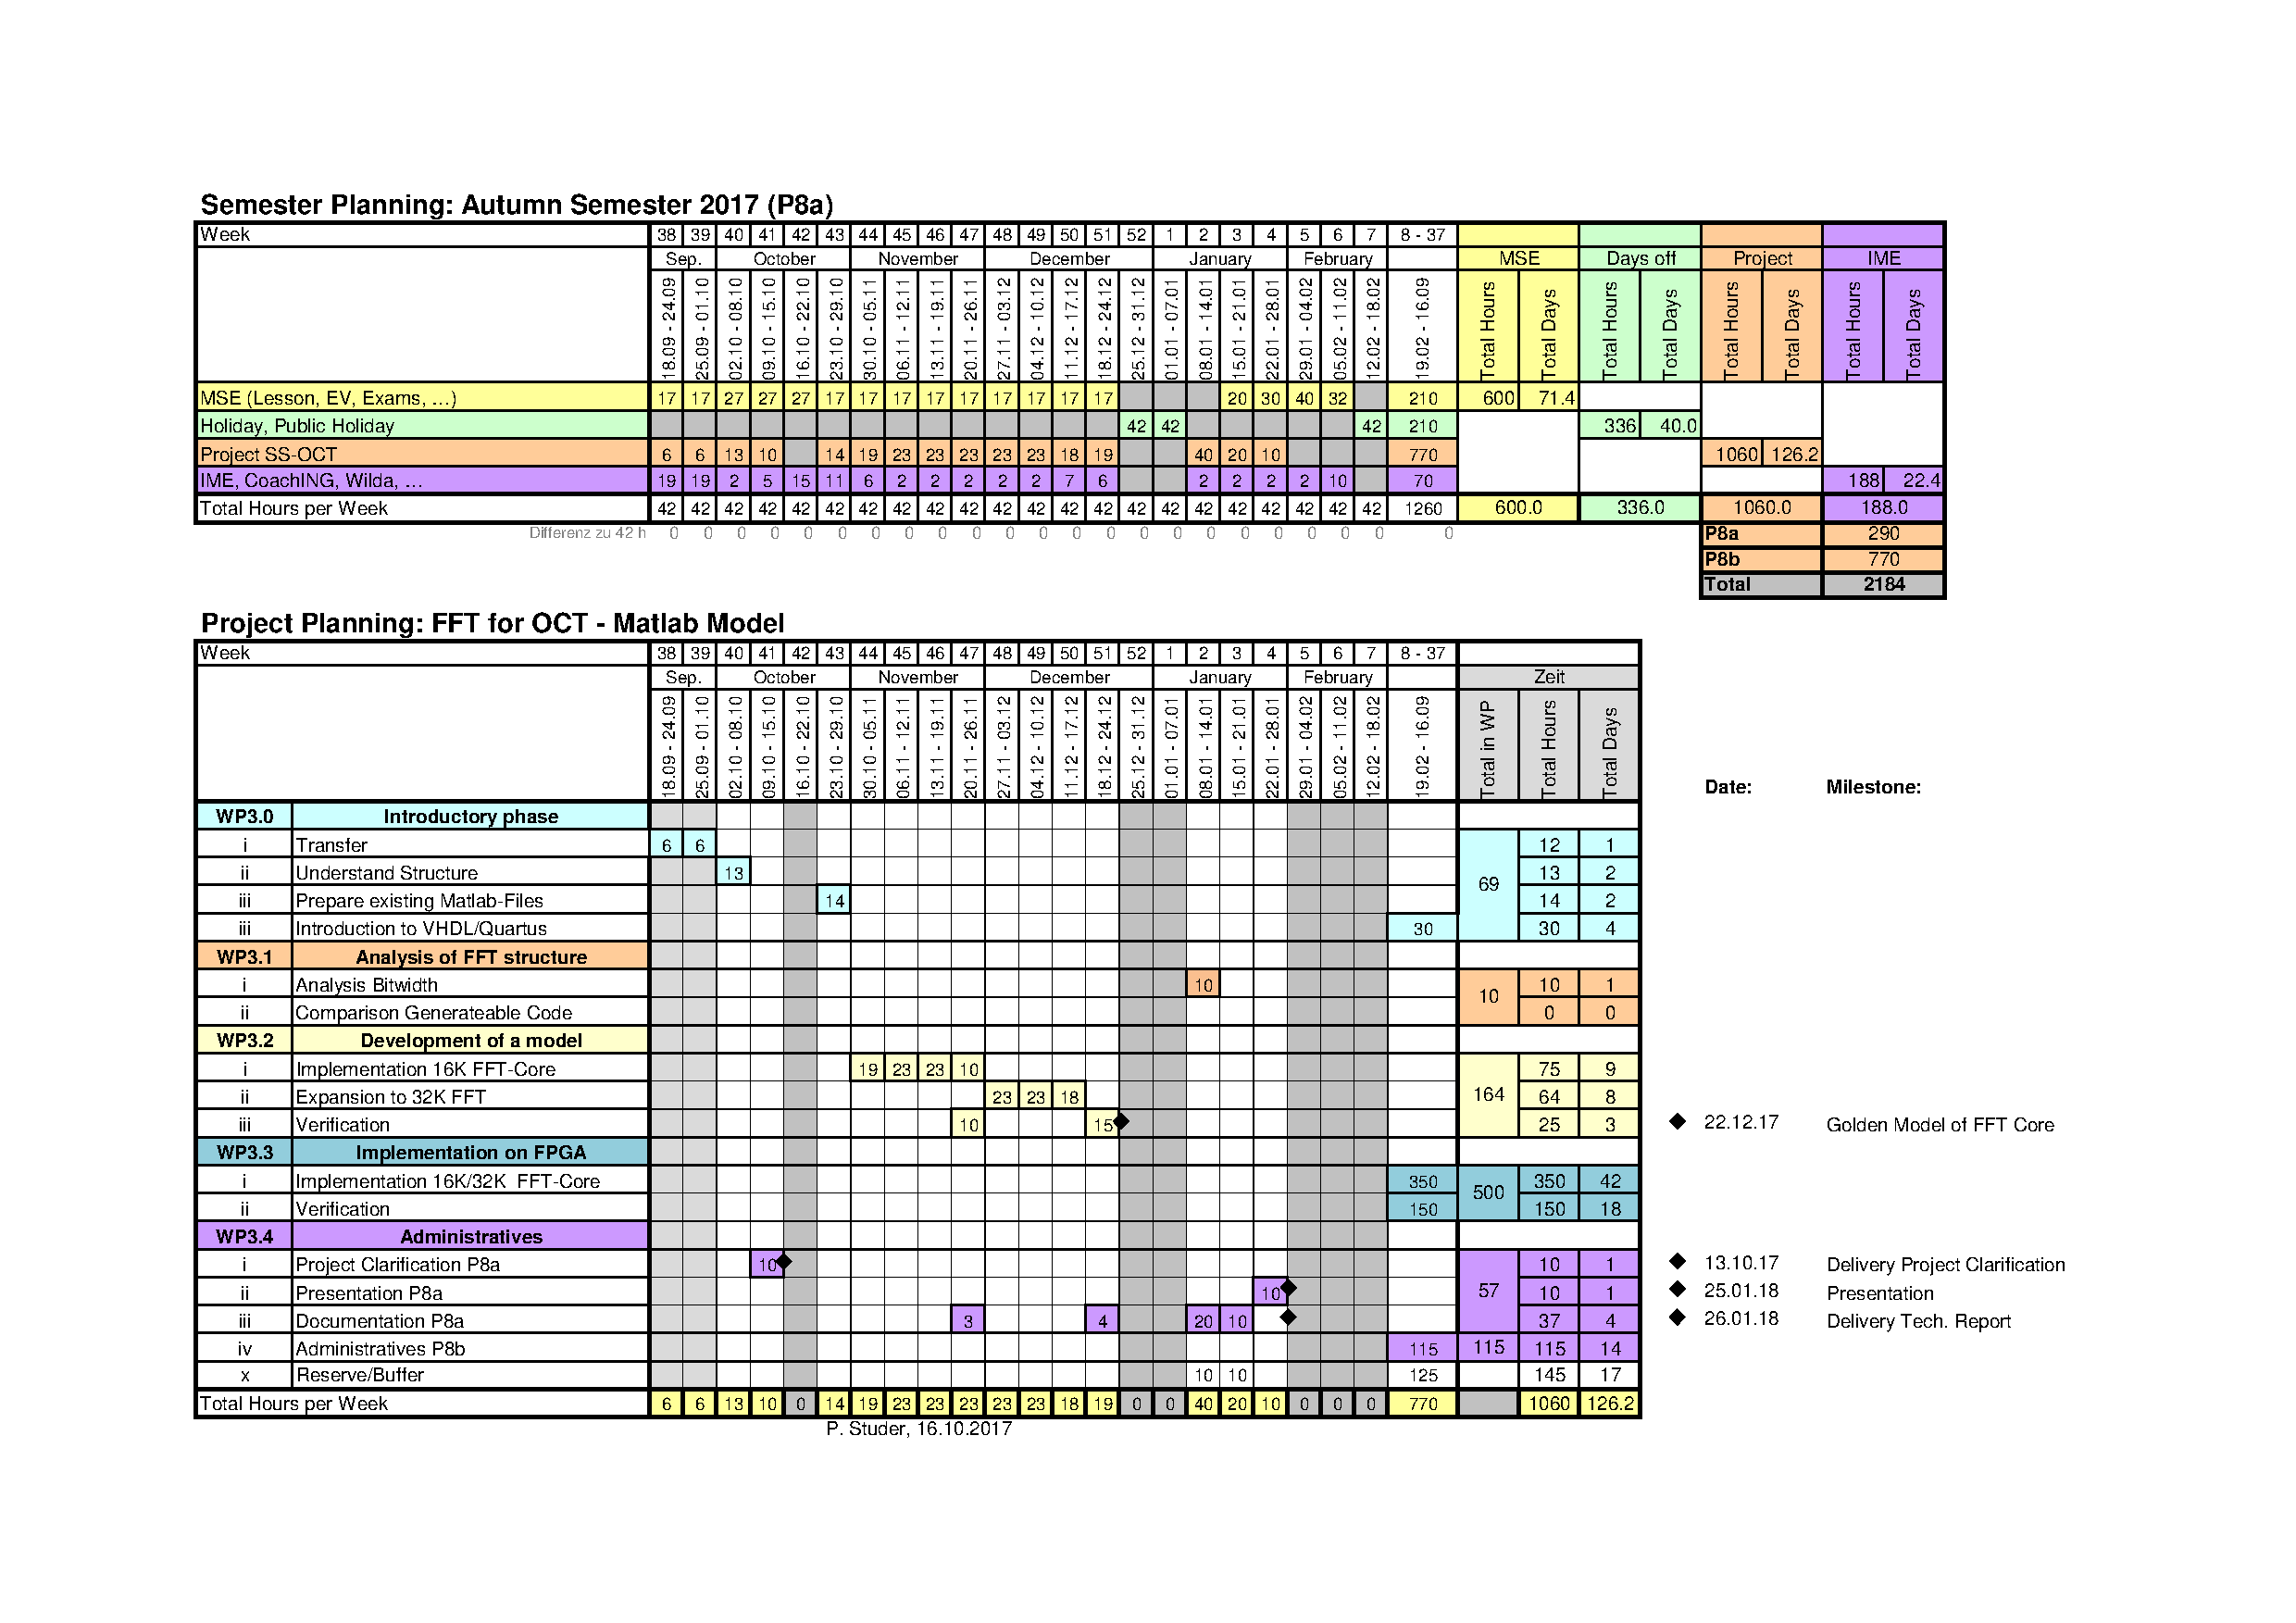
\includepdf[pages={1},nup=1x1,landscape=true,scale=0.85,offset=10 -40,pagecommand={\section{Eingefügte PDF-Tabelle}\label{app:Timetable}\thispagestyle{myheadings}}]{appendix/timeline_example.pdf} \newpage
%%Bei mehrseitigen Dokumenten die folgenden Seiten ohne Überschrift:
%\includepdf[pages={2-5},nup=1x1,landscape=true,scale=0.85,offset=0 -20,pagecommand={\thispagestyle{myheadings}}]{appendix/timeline_example.pdf} \newpage

\section{MATLAB-Code Snippets}
\lstinputlisting{appendix/code/matlab.m}


\end{appendix}


%%---NOTES for DEBUG---------------------------------------------------------------------
\ifdraft{%Do this only if mode=draft
%%requires \usepackage{todonotes})
\newpage
\listoftodos[\section{Todo-Notes}]
\clearpage
}
{%Do this only if mode=final
}
\end{document}
